\documentclass{standalone}
\usepackage{tikz}
\usetikzlibrary{patterns, positioning}


\begin{document}
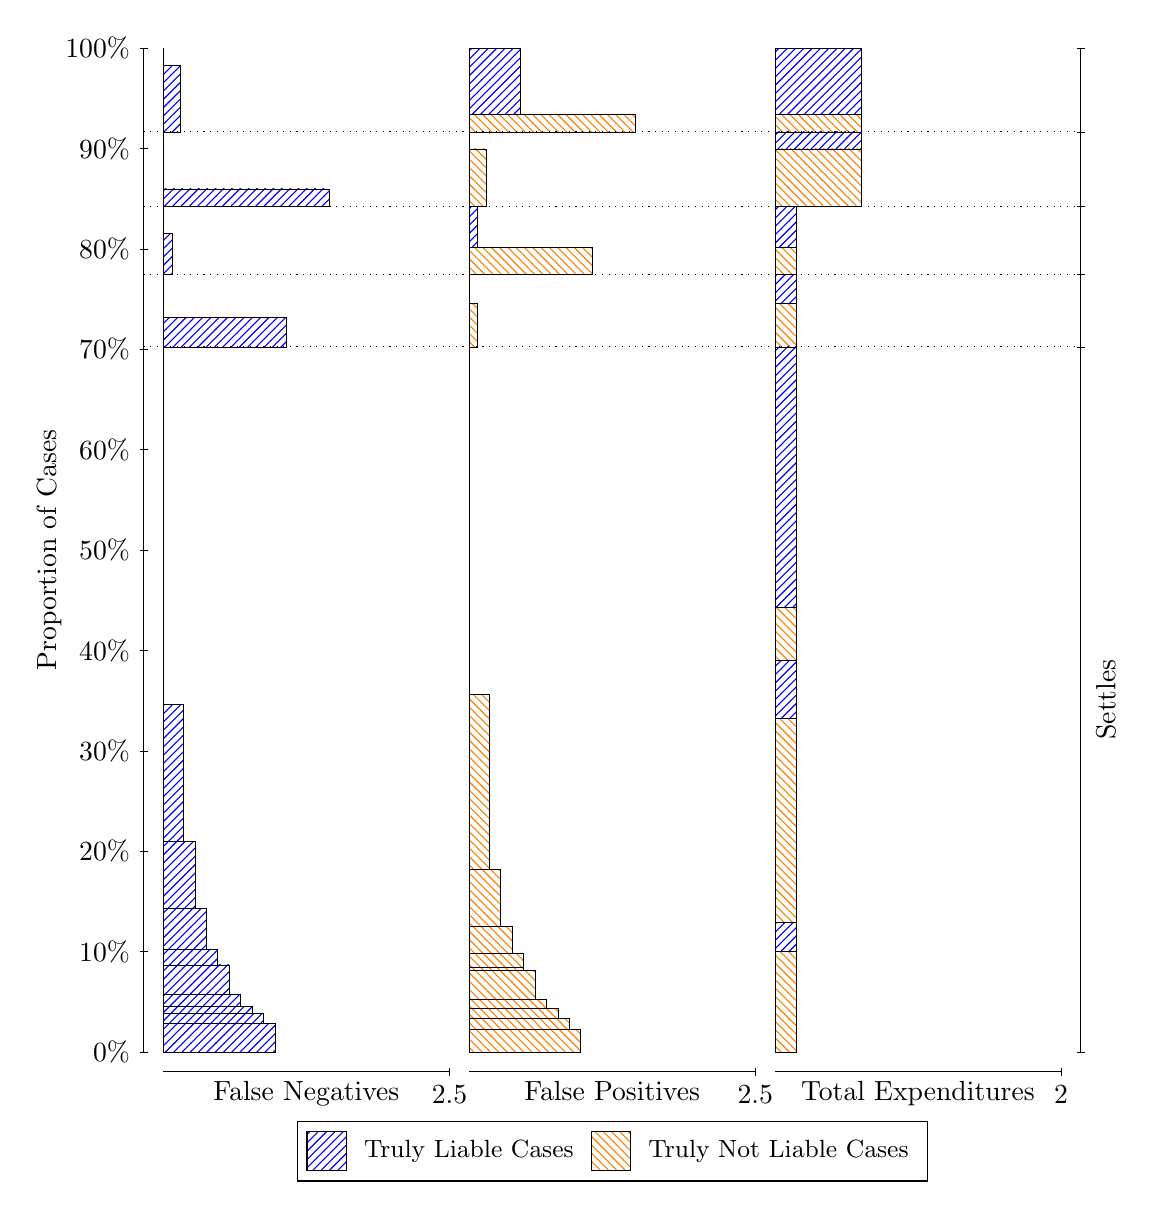
\begin{tikzpicture}
\draw[black, very thin] (1.5,1.75) -- (1.5,14.5);
\node[rotate=90, text=black, anchor=center] at (0.3, 8.125) {Proportion of Cases};
\draw[black, very thin] (1.45,1.75) -- (1.55,1.75);
\node[text=black, anchor=east] at (1.45, 1.75) {0\%};
\draw[black, very thin] (1.45,3.025) -- (1.55,3.025);
\node[text=black, anchor=east] at (1.45, 3.025) {10\%};
\draw[black, very thin] (1.45,4.3) -- (1.55,4.3);
\node[text=black, anchor=east] at (1.45, 4.3) {20\%};
\draw[black, very thin] (1.45,5.575) -- (1.55,5.575);
\node[text=black, anchor=east] at (1.45, 5.575) {30\%};
\draw[black, very thin] (1.45,6.85) -- (1.55,6.85);
\node[text=black, anchor=east] at (1.45, 6.85) {40\%};
\draw[black, very thin] (1.45,8.125) -- (1.55,8.125);
\node[text=black, anchor=east] at (1.45, 8.125) {50\%};
\draw[black, very thin] (1.45,9.4) -- (1.55,9.4);
\node[text=black, anchor=east] at (1.45, 9.4) {60\%};
\draw[black, very thin] (1.45,10.675) -- (1.55,10.675);
\node[text=black, anchor=east] at (1.45, 10.675) {70\%};
\draw[black, very thin] (1.45,11.95) -- (1.55,11.95);
\node[text=black, anchor=east] at (1.45, 11.95) {80\%};
\draw[black, very thin] (1.45,13.225) -- (1.55,13.225);
\node[text=black, anchor=east] at (1.45, 13.225) {90\%};
\draw[black, very thin] (1.45,14.5) -- (1.55,14.5);
\node[text=black, anchor=east] at (1.45, 14.5) {100\%};

\draw[black, very thin] (13.4,1.75) -- (13.4,14.5);
\draw[black, very thin] (13.35,1.75) -- (13.45,1.75);
\node[anchor=west] at (13.35, 1.75) {};
\draw[black, very thin] (13.35,10.704) -- (13.45,10.704);
\node[anchor=west] at (13.35, 10.704) {};
\draw[black, very thin] (13.35,11.625) -- (13.45,11.625);
\node[anchor=west] at (13.35, 11.625) {};
\draw[black, very thin] (13.35,12.492) -- (13.45,12.492);
\node[anchor=west] at (13.35, 12.492) {};
\draw[black, very thin] (13.35,13.436) -- (13.45,13.436);
\node[anchor=west] at (13.35, 13.436) {};
\draw[black, very thin] (13.35,14.5) -- (13.45,14.5);
\node[anchor=west] at (13.35, 14.5) {};

\draw[black, very thin, pattern color=blue, pattern=north east lines] (1.75,1.75) rectangle (3.167,2.1136);
\draw[black, very thin, pattern color=blue, pattern=north east lines] (1.75,2.1136) rectangle (3.0217,2.241);
\draw[black, very thin, pattern color=blue, pattern=north east lines] (1.75,2.241) rectangle (2.8763,2.3303);
\draw[black, very thin, pattern color=blue, pattern=north east lines] (1.75,2.3303) rectangle (2.731,2.486);
\draw[black, very thin, pattern color=blue, pattern=north east lines] (1.75,2.486) rectangle (2.5857,2.8573);
\draw[black, very thin, pattern color=blue, pattern=north east lines] (1.75,2.8573) rectangle (2.4403,3.0527);
\draw[black, very thin, pattern color=blue, pattern=north east lines] (1.75,3.0527) rectangle (2.295,3.5698);
\draw[black, very thin, pattern color=blue, pattern=north east lines] (1.75,3.5698) rectangle (2.1497,4.4216);
\draw[black, very thin, pattern color=blue, pattern=north east lines] (1.75,4.4216) rectangle (2.0043,6.1662);
\draw[black, very thin, pattern color=orange, pattern=north west lines] (1.75,6.1662) rectangle (1.75,10.704);
\draw[black, very thin, pattern color=blue, pattern=north east lines] (1.75,10.704) rectangle (3.3123,11.075);
\draw[black, very thin, pattern color=orange, pattern=north west lines] (1.75,11.075) rectangle (1.75,11.625);
\draw[black, very thin, pattern color=blue, pattern=north east lines] (1.75,11.625) rectangle (1.859,12.149);
\draw[black, very thin, pattern color=orange, pattern=north west lines] (1.75,12.149) rectangle (1.75,12.492);
\draw[black, very thin, pattern color=blue, pattern=north east lines] (1.75,12.492) rectangle (3.8573,12.71);
\draw[black, very thin, pattern color=orange, pattern=north west lines] (1.75,12.71) rectangle (1.75,13.436);
\draw[black, very thin, pattern color=blue, pattern=north east lines] (1.75,13.436) rectangle (1.968,14.281);
\draw[black, very thin, pattern color=orange, pattern=north west lines] (1.75,14.281) rectangle (1.75,14.5);
\draw[black, very thin, pattern color=orange, pattern=north west lines] (5.6333,1.75) rectangle (7.0503,2.0344);
\draw[black, very thin, pattern color=orange, pattern=north west lines] (5.6333,2.0344) rectangle (6.905,2.1801);
\draw[black, very thin, pattern color=orange, pattern=north west lines] (5.6333,2.1801) rectangle (6.7597,2.3013);
\draw[black, very thin, pattern color=orange, pattern=north west lines] (5.6333,2.3013) rectangle (6.6143,2.4195);
\draw[black, very thin, pattern color=orange, pattern=north west lines] (5.6333,2.4195) rectangle (6.469,2.7874);
\draw[black, very thin, pattern color=orange, pattern=north west lines] (5.6333,2.7874) rectangle (6.3237,2.8275);
\draw[black, very thin, pattern color=orange, pattern=north west lines] (5.6333,2.8275) rectangle (6.3237,3.003);
\draw[black, very thin, pattern color=orange, pattern=north west lines] (5.6333,3.003) rectangle (6.1783,3.3424);
\draw[black, very thin, pattern color=orange, pattern=north west lines] (5.6333,3.3424) rectangle (6.033,4.0641);
\draw[black, very thin, pattern color=orange, pattern=north west lines] (5.6333,4.0641) rectangle (5.8877,6.2879);
\draw[black, very thin, pattern color=blue, pattern=north east lines] (5.6333,6.2879) rectangle (5.6333,10.704);
\draw[black, very thin, pattern color=orange, pattern=north west lines] (5.6333,10.704) rectangle (5.7423,11.254);
\draw[black, very thin, pattern color=blue, pattern=north east lines] (5.6333,11.254) rectangle (5.6333,11.625);
\draw[black, very thin, pattern color=orange, pattern=north west lines] (5.6333,11.625) rectangle (7.1957,11.968);
\draw[black, very thin, pattern color=blue, pattern=north east lines] (5.6333,11.968) rectangle (5.7423,12.492);
\draw[black, very thin, pattern color=orange, pattern=north west lines] (5.6333,12.492) rectangle (5.8513,13.218);
\draw[black, very thin, pattern color=blue, pattern=north east lines] (5.6333,13.218) rectangle (5.6333,13.436);
\draw[black, very thin, pattern color=orange, pattern=north west lines] (5.6333,13.436) rectangle (7.7407,13.654);
\draw[black, very thin, pattern color=blue, pattern=north east lines] (5.6333,13.654) rectangle (6.2873,14.5);
\draw[black, very thin, pattern color=orange, pattern=north west lines] (9.5167,1.75) rectangle (9.7892,3.0268);
\draw[black, very thin, pattern color=blue, pattern=north east lines] (9.5167,3.0268) rectangle (9.7892,3.3991);
\draw[black, very thin, pattern color=orange, pattern=north west lines] (9.5167,3.3991) rectangle (9.7892,5.9908);
\draw[black, very thin, pattern color=blue, pattern=north east lines] (9.5167,5.9908) rectangle (9.7892,6.7257);
\draw[black, very thin, pattern color=orange, pattern=north west lines] (9.5167,6.7257) rectangle (9.7892,7.3952);
\draw[black, very thin, pattern color=blue, pattern=north east lines] (9.5167,7.3952) rectangle (9.7892,10.704);
\draw[black, very thin, pattern color=orange, pattern=north west lines] (9.5167,10.704) rectangle (9.7892,11.254);
\draw[black, very thin, pattern color=blue, pattern=north east lines] (9.5167,11.254) rectangle (9.7892,11.625);
\draw[black, very thin, pattern color=orange, pattern=north west lines] (9.5167,11.625) rectangle (9.7892,11.968);
\draw[black, very thin, pattern color=blue, pattern=north east lines] (9.5167,11.968) rectangle (9.7892,12.492);
\draw[black, very thin, pattern color=orange, pattern=north west lines] (9.5167,12.492) rectangle (10.607,13.218);
\draw[black, very thin, pattern color=blue, pattern=north east lines] (9.5167,13.218) rectangle (10.607,13.436);
\draw[black, very thin, pattern color=orange, pattern=north west lines] (9.5167,13.436) rectangle (10.607,13.654);
\draw[black, very thin, pattern color=blue, pattern=north east lines] (9.5167,13.654) rectangle (10.607,14.5);
\draw[black, dotted] (1.5,10.704) -- (13.4,10.704);
\draw[black, dotted] (1.5,11.625) -- (13.4,11.625);
\draw[black, dotted] (1.5,12.492) -- (13.4,12.492);
\draw[black, dotted] (1.5,13.436) -- (13.4,13.436);
\draw[black, very thin] (1.75,1.5) -- (5.3833,1.5);
\node[text=black, anchor=north] at (3.5667, 1.5) {False Negatives};
\draw[black, very thin] (5.3833,1.45) -- (5.3833,1.55);
\node[text=black, anchor=north] at (5.3833, 1.45) {2.5};

\draw[black, very thin] (5.6333,1.5) -- (9.2667,1.5);
\node[text=black, anchor=north] at (7.45, 1.5) {False Positives};
\draw[black, very thin] (9.2667,1.45) -- (9.2667,1.55);
\node[text=black, anchor=north] at (9.2667, 1.45) {2.5};

\draw[black, very thin] (9.5167,1.5) -- (13.15,1.5);
\node[text=black, anchor=north] at (11.333, 1.5) {Total Expenditures};
\draw[black, very thin] (13.15,1.45) -- (13.15,1.55);
\node[text=black, anchor=north] at (13.15, 1.45) {2};

\node[text=black, centered, rotate=90] at (13.72, 6.227) {Settles};





\draw (7.449999999999999,1.5) node[draw=none] (baseCoordinate) {};
\begin{scope}[align=center]
        \matrix[scale=0.5, draw=black, below=0.5cm of baseCoordinate, nodes={draw}, column sep=0.1cm]{
            \node[rectangle, draw, minimum width=0.5cm, minimum height=0.5cm, pattern color=blue, pattern=north east lines] {}; &
            \node[draw=none, font=\small, text=black] (B) {Truly Liable Cases}; &
            \node[rectangle, draw, minimum width=0.5cm, minimum height=0.5cm, pattern color=orange, pattern=north west lines] {}; &
            \node[draw=none, font=\small, text=black] (B) {Truly Not Liable Cases}; \\
            };
\end{scope}

\end{tikzpicture}
\end{document}